\documentclass[conference]{IEEEtran}
\IEEEoverridecommandlockouts
\usepackage{cite}
\usepackage{amsmath,amssymb,amsfonts}
\usepackage{algorithmic}
\usepackage{graphicx}
\usepackage{textcomp}
\usepackage{xcolor}
\usepackage{array}
\usepackage{booktabs}
\usepackage{multirow}
\usepackage{url}
\usepackage[utf8]{inputenc}
\usepackage[spanish]{babel}
\usepackage{tikz}
\usetikzlibrary{shapes.geometric, arrows.meta, positioning}

% Define TikZ styles after babel to avoid conflicts
\tikzset{
    startstop/.style = {rectangle, rounded corners, minimum width=2.5cm, minimum height=0.8cm, text centered, draw=black, fill=blue!15},
    process/.style = {rectangle, minimum width=2.5cm, minimum height=0.8cm, text centered, draw=black, fill=orange!20},
    decision/.style = {diamond, minimum width=2cm, minimum height=1cm, text centered, draw=black, fill=yellow!15},
    arrow/.style = {thick, ->, >=stealth}
}

\def\BibTeX{{\rm B\kern-.05em{\sc i\kern-.025em b}\kern-.08em
    T\kern-.1667em\lower.7ex\hbox{E}\kern-.125emX}}

\begin{document}

\title{Análisis Comparativo de Optimización por Enjambre de Partículas (PSO) y Optuna para la Predicción del Rendimiento Académico en Educación Básica Peruana}

\author{\IEEEauthorblockN{Beatriz Umiña Machaca}
\IEEEauthorblockA{\textit{Facultad de Ingeniería Estadística e Informática} \\
\textit{Universidad Nacional del Altiplano Puno}\\
Puno, Perú \\
beatrizuminamachaca@gmail.com}
}

\maketitle

\begin{abstract}
Este artículo presenta una metodología comparativa para predecir el rendimiento académico estudiantil mediante técnicas de Inteligencia de Enjambre, específicamente el algoritmo de Optimización por Enjambre de Partículas (PSO), aplicado al ajuste de hiperparámetros de modelos de aprendizaje automático. El estudio se basa en un conjunto de datos reales provenientes de la Evaluación Muestral 2022 del Ministerio de Educación del Perú, que comprende 7839 registros de estudiantes de sexto grado de primaria, incluyendo puntajes en las pruebas estandarizadas de lectura y matemática, así como variables socioeconómicas, demográficas y contextuales de las 25 regiones del país. El enfoque propuesto con PSO se compara con la optimización bayesiana utilizando el framework Optuna mediante validación cruzada de 5 pliegues para ambas materias evaluadas. Los resultados demuestran rendimiento estadísticamente equivalente entre ambos métodos en ambas áreas curriculares. En lectura, el modelo optimizado con PSO alcanzó un Error Cuadrático Medio (MSE) de 4872 ± 106 y un coeficiente de determinación (R²) de 0.203 ± 0.016, mientras que Optuna logró un MSE de 4872 ± 112 y un R² de 0.203 ± 0.016. En matemática, PSO obtuvo MSE de 6650 ± 261 y R² de 0.154 ± 0.021, comparado con Optuna que alcanzó MSE de 6651 ± 262 y R² de 0.154 ± 0.021. Las pruebas t de Student confirmaron ausencia de diferencias estadísticamente significativas (p > 0.05) en ambas materias. El análisis de eficiencia computacional reveló patrones diferenciados por materia: en lectura, PSO demostró mayor eficiencia utilizando 88 árboles versus 177 de Optuna, mientras que en matemática, Optuna fue más eficiente con 152 árboles frente a 180 de PSO. El análisis territorial evidenció desigualdades educativas críticas, con departamentos costeros como Callao (575.29 puntos), Tacna (565.47) y Lima (561.29) superando significativamente a regiones amazónicas como Loreto (453.50), San Martín (490.45) y Huánuco (497.41), generando una brecha territorial de 121.79 puntos equivalente a aproximadamente 1.7 años de escolaridad. El estudio concluye que tanto PSO como la optimización bayesiana representan alternativas metodológicamente equivalentes para el ajuste de hiperparámetros en contextos educativos, con la selección del método dependiendo de los recursos computacionales disponibles y la materia específica. PSO ofrece mayor simplicidad de implementación y eficiencia en lectura, mientras Optuna proporciona mayor sofisticación metodológica y eficiencia en matemática. Esta equivalencia resulta especialmente relevante para instituciones educativas con recursos computacionales limitados, permitiendo selección basada en criterios operativos específicos y contribuyendo al desarrollo de sistemas de alerta temprana para identificación de estudiantes en riesgo académico.
\end{abstract}

\begin{IEEEkeywords}
Minería de datos educativos, predicción del rendimiento académico, optimización por enjambre de partículas, metaheurísticas, ajuste de hiperparámetros, evaluación educativa peruana, modelos de aprendizaje automático, validación cruzada, análisis territorial educativo
\end{IEEEkeywords}

\section{Introducción}

La Minería de Datos Educativos ha emergido como una disciplina fundamental para analizar grandes volúmenes de información provenientes de sistemas educativos, utilizando técnicas estadísticas avanzadas y algoritmos de aprendizaje automático para detectar variables críticas que influyen en el rendimiento académico estudiantil \cite{romero2020educational}. Los modelos predictivos en educación proporcionan evidencia empírica para el desarrollo de políticas públicas efectivas y habilitan intervenciones tempranas mediante la identificación oportuna de estudiantes en riesgo académico \cite{baker2014educational}.

El sistema educativo peruano presenta brechas socioeconómicas significativas y heterogeneidades regionales que limitan el rendimiento académico, evidenciadas en disparidades territoriales que superan los 120 puntos entre departamentos costeros y amazónicos. Los datos de evaluaciones nacionales como la Evaluación Muestral 2022 constituyen una fuente estratégica para aplicar técnicas de minería de datos educativos en el contexto de estas desigualdades estructurales. El desarrollo de modelos predictivos robustos enfrenta desafíos metodológicos críticos, incluyendo la optimización de hiperparámetros y la selección rigurosa de variables predictivas que permitan identificar patrones territoriales y socioeconómicos determinantes del rendimiento estudiantil \cite{dutt2017systematic}.

En el ámbito de optimización de hiperparámetros, han surgido dos enfoques principales con aplicaciones prometedoras en contextos educativos. Los algoritmos bioinspirados, especialmente la Inteligencia de Enjambre mediante Optimización por Enjambre de Partículas (PSO), realizan búsquedas eficientes en espacios multidimensionales complejos con requisitos computacionales moderados \cite{kennedy1995particle}. Paralelamente, los métodos de optimización bayesiana, implementados en frameworks como Optuna, utilizan modelos probabilísticos para guiar búsquedas futuras de manera más eficiente mediante algoritmos sofisticados como Tree-structured Parzen Estimator (TPE) \cite{bergstra2013making}.

La Optimización por Enjambre de Partículas se ha consolidado como herramienta efectiva para el ajuste de modelos debido a su simplicidad computacional, mínima dependencia del cálculo de derivadas, y capacidad para escapar de óptimos locales \cite{kennedy1995particle}. Esta característica resulta particularmente relevante para instituciones educativas con recursos computacionales limitados. Optuna ha emergido como framework líder mediante su implementación del algoritmo TPE, distinguiéndose por su convergencia rápida, capacidad de poda automática y optimización adaptativa que puede resultar más eficiente en contextos específicos \cite{akiba2019optuna}.

Este estudio compara sistemáticamente PSO contra Optuna utilizando datos reales de la Evaluación Muestral 2022 de estudiantes peruanos de sexto grado, evaluando la efectividad de ambos métodos en la predicción del rendimiento académico en lectura y matemática. La investigación contribuye al campo de optimización metaheurística y análisis educativo orientado a datos, proporcionando evidencia empírica sobre la equivalencia metodológica entre enfoques bioinspirados y bayesianos. El análisis territorial incorporado permite identificar patrones geográficos críticos que requieren intervenciones diferenciadas, ofreciendo recomendaciones prácticas para investigadores y gestores educativos en contextos de recursos limitados.

En este contexto, surge la pregunta de investigación: ¿Cuál es la efectividad comparativa de la Optimización por Enjambre de Partículas (PSO) frente a la optimización bayesiana (Optuna) en términos de precisión predictiva y eficiencia computacional para la predicción del rendimiento académico en lectura y matemática con datos educativos peruanos, y qué implicaciones territoriales emergen del análisis predictivo?

\section{Revisión de Literatura}

La Optimización por Enjambre de Partículas (PSO), propuesta por Kennedy y Eberhart \cite{kennedy1995particle}, ha demostrado efectividad en tareas de optimización continua y ajuste de modelos en dominios complejos \cite{liu2020improved}. En el ámbito educativo, PSO ha sido utilizada para predecir rendimiento académico en plataformas virtuales \cite{zhang2021learning} y optimizar modelos de clasificación para detectar estudiantes en riesgo \cite{sultana2021pso}. En América Latina, González et al. \cite{gonzalez2023edmcolombia} aplicaron PSO a datos escolares colombianos obteniendo mejoras notables en precisión predictiva.

Paralelamente, la optimización bayesiana ha revolucionado el ajuste de hiperparámetros mediante frameworks como Optuna, que implementa el algoritmo Tree-structured Parzen Estimator (TPE) \cite{akiba2019optuna}. Optuna se distingue por su convergencia rápida, poda automática de configuraciones no prometedoras, e integración con librerías de aprendizaje automático \cite{feurer2019hyperparameter}. Su aplicación en entornos educativos ha mostrado resultados prometedores en predicción de rendimiento estudiantil \cite{yang2022optunaed}.

La Minería de Datos Educativos (EDM) ha emergido como disciplina clave para descubrir patrones que permitan predecir resultados y personalizar experiencias de aprendizaje \cite{romero2020educational, baker2014educational}. En América Latina, la implementación de EDM enfrenta limitaciones técnicas e institucionales \cite{pena2014educational}, requiriendo contextualización según realidades sociales específicas. Los estudios sobre desigualdades educativas territoriales han documentado persistentes brechas de rendimiento entre regiones urbanas y rurales \cite{williamson2020datafication}.

En el contexto peruano, los datos de la Evaluación Muestral 2022 \cite{minedu2022em} ofrecen potencial significativo para modelos predictivos avanzados. La comparación entre PSO y Optuna resulta particularmente relevante dado que representan filosofías de optimización complementarias: simplicidad de implementación versus sofisticación metodológica, especialmente importante en contextos educativos con recursos limitados.

\section{Metodología}

\subsection{Conjunto de Datos y Variables}
Este estudio utiliza microdatos de la Evaluación Muestral 2022 del Ministerio de Educación del Perú, específicamente el conjunto correspondiente a sexto grado de primaria. La muestra comprende 7839 estudiantes distribuidos en las 25 regiones del país, garantizando cobertura geográfica representativa de zonas urbanas y rurales \cite{minedu2022em}. Las variables objetivo corresponden a los puntajes estandarizados de lectura y matemática, medidos en escala continua de 0 a 1000 puntos.El conjunto de datos incluye seis variables predictoras categóricas que permiten analizar tanto factores individuales como territoriales que influyen en el rendimiento académico: sexo (Hombre, Mujer), lengua materna (Castellano, Quechua, Aimara, otras), gestión educativa (Estatal, No estatal), zona geográfica (Rural, Urbana), nivel socioeconómico (Muy bajo, Bajo, Medio, Alto), y departamento de residencia (25 categorías).

\begin{table}[htbp]
\caption{Variables del conjunto de datos}
\resizebox{\columnwidth}{!}{
\begin{tabular}{lll}
\hline
\textbf{Variable} & \textbf{Tipo} & \textbf{Descripción} \\
\hline
\texttt{puntaje\_lectura} & Numérica & Puntaje lectura (0-1000) \\
\texttt{puntaje\_matematica} & Numérica & Puntaje matemática (0-1000) \\
\texttt{sexo} & Categórica & Género del estudiante \\
\texttt{lengua\_materna} & Categórica & Idioma principal del hogar \\
\texttt{gestion} & Categórica & Tipo institución (Estatal/No estatal) \\
\texttt{zona} & Categórica & Ubicación geográfica (Rural/Urbana) \\
\texttt{nivel\_socioeconomico} & Categórica & Estrato socioeconómico (4 niveles) \\
\texttt{departamento} & Categórica & Departamento de residencia (25 categorías) \\
\hline
\end{tabular}
}
\label{tab:variables}
\end{table}

\subsection{Modelos de Optimización y Validación}
Se empleó Random Forest como algoritmo base debido a su robustez ante variables categóricas mixtas, resistencia al sobreajuste, y capacidad para manejar interacciones no lineales entre variables predictoras. Los hiperparámetros optimizados fueron el número de árboles (\texttt{n\_estimators}) con rango [10, 200] y la profundidad máxima (\texttt{max\_depth}) con rango [3, 20].

Para la optimización se implementaron dos enfoques metodológicos. PSO se configuró con 20 partículas y 50 iteraciones máximas, utilizando la librería \texttt{pyswarm} con parámetros estándar de inercia y aceleración. Optuna se implementó mediante el algoritmo Tree-structured Parzen Estimator con 50 evaluaciones, aplicando poda automática para configuraciones no prometedoras.El algoritmo PSO implementa los principios fundamentales de inteligencia de enjambre donde cada partícula representa una solución candidata en el espacio de hiperparámetros. La Figura~\ref{fig:pso_algorithm} ilustra el proceso de optimización por enjambre de partículas desarrollado para este estudio.

\begin{figure}[htbp]
\centerline{
\begin{tikzpicture}[node distance=1.9cm, scale=0.9, transform shape]

\node (inicio) [startstop] {Inicializar PSO};
\node (generar) [process, below of=inicio] {Generar 20\\partículas aleatorias};
\node (evaluar) [process, below of=generar] {Evaluar fitness\\cada partícula};
\node (actualizarp) [process, below of=evaluar] {Actualizar pbest\\de cada partícula};
\node (actualizarg) [process, below of=actualizarp] {Actualizar gbest\\del enjambre};
\node (velocidad) [process, below of=actualizarg] {Calcular nueva\\velocidad};
\node (posicion) [process, below of=velocidad] {Actualizar\\posición};
\node (criterio) [decision, below of=posicion] {Criterio\\parada?};
\node (resultado) [startstop, right of=criterio, node distance=3cm] {Retornar gbest\\óptimo};

\draw [arrow] (inicio) -- (generar);
\draw [arrow] (generar) -- (evaluar);
\draw [arrow] (evaluar) -- (actualizarp);
\draw [arrow] (actualizarp) -- (actualizarg);
\draw [arrow] (actualizarg) -- (velocidad);
\draw [arrow] (velocidad) -- (posicion);
\draw [arrow] (posicion) -- (criterio);
\draw [arrow] (criterio) -- node[above] {Si} (resultado);
\draw [arrow] (criterio.west) -- ++(-1.5,0) |- node[left] {No} (evaluar.west);
\end{tikzpicture}
}
\caption{Algoritmo de Optimización por Enjambre de Partículas (PSO) para ajuste de hiperparámetros}
\label{fig:pso_algorithm}
\end{figure}

El proceso PSO inicia generando 20 partículas con posiciones aleatorias en el espacio bidimensional de hiperparámetros (\texttt{n\_estimators}, \texttt{max\_depth}). Cada partícula mantiene su mejor posición histórica (pbest) y el enjambre conserva la mejor posición global (gbest). En cada iteración, las partículas actualizan su velocidad considerando tres componentes: inercia de movimiento previo, atracción hacia su mejor experiencia personal, y atracción hacia la mejor experiencia colectiva del enjambre. El algoritmo continúa hasta alcanzar convergencia o completar 50 iteraciones máximas.Se implementó validación cruzada estratificada de 5 pliegues para garantizar robustez estadística \cite{kohavi1995study}. La función objetivo minimizada corresponde al error cuadrático medio promedio:

\begin{equation}
\text{MSE}_{CV} = \frac{1}{k} \sum_{i=1}^{k} \text{MSE}_i
\end{equation}

donde $k=5$ representa el número de pliegues. Las métricas finales incluyen promedio y desviación estándar del MSE y coeficiente de determinación ($R^2$) para cada algoritmo y materia. La significancia estadística se evaluó mediante pruebas t de Student para muestras pareadas \cite{dietterich1998approximate} con $\alpha = 0.05$.

\subsection{Implementación y Análisis Territorial}
La implementación se realizó en Python utilizando \texttt{scikit-learn} para Random Forest, \texttt{pyswarm} para PSO, \texttt{optuna} para optimización bayesiana, y \texttt{scipy} para análisis estadístico. El procesamiento de variables categóricas empleó \texttt{LabelEncoder} manteniendo consistencia en la codificación. Todas las evaluaciones utilizaron semilla aleatoria fija (\texttt{random\_state=42}) garantizando reproducibilidad.Complementariamente, se desarrolló análisis territorial descriptivo identificando patrones geográficos en rendimiento académico. Los 25 departamentos se categorizaron en cuatro niveles de riesgo educativo basados en cuartiles de puntaje promedio en lectura: Óptimo (Q4), Medio (Q3), Alto (Q2), y Crítico (Q1). Esta categorización permite identificar regiones prioritarias para intervenciones educativas y cuantificar brechas territoriales en el sistema educativo peruano.

\section{Resultados y Análisis}

\subsection{Estadísticas Descriptivas}
A continuación se presentan las estadísticas descriptivas para los puntajes de lectura y matemática de los estudiantes evaluados. Se calculó la media, desviación estándar, valores mínimo y máximo, así como los percentiles para caracterizar la distribución del rendimiento académico en ambas materias.




\begin{table}[htbp]
\caption{Estadísticas descriptivas de los puntajes de lectura y matemática}
\centering
\resizebox{\columnwidth}{!}{
\begin{tabular}{lcc}
\hline
\textbf{Estadística} & \textbf{Lectura} & \textbf{Matemática} \\
\hline
Cantidad de estudiantes (n)     & 7839    & 7839     \\
Media (\textit{mean})           & 541.17  & 527.69   \\
Desviación estándar (\textit{std}) & 78.20   & 88.68    \\
Mínimo                          & 185.54  & 200.51   \\
Percentil 25 (Q1)               & 490.45  & 472.06   \\
Mediana (Q2)                    & 539.99  & 524.67   \\
Percentil 75 (Q3)               & 591.73  & 579.35   \\
Máximo                          & 785.74  & 879.81   \\
Coeficiente de variación (CV)  & 0.1445  & 0.1681   \\
\hline
\end{tabular}
}
\label{tab:estadisticas_descriptivas}
\end{table}


La media en lectura (541.17) supera a la de matemática (527.69), indicando que los estudiantes se desempeñaron mejor en comprensión lectora. La mayor desviación estándar en matemática (88.68 vs 78.20) sugiere mayor variabilidad entre estudiantes en esta área. El coeficiente de variación confirma que los resultados en lectura son más homogéneos, mientras que matemática presenta mayor dispersión relativa, posiblemente reflejando diferencias en la complejidad conceptual de ambas materias.


\begin{figure}[htbp]
\centerline{
\includegraphics[width=0.45\textwidth]{grafica1_distribucion.png}}
\caption{Distribución de puntajes en lectura y matemática}
\label{fig:distribucion_puntajes}
\end{figure}
La distribución de puntajes presenta forma aproximadamente normal en ambas materias, con concentración entre 450 y 600 puntos. Matemática evidencia mayor dispersión y presencia de valores extremos, confirmando la heterogeneidad observada en las estadísticas descriptivas.

\begin{figure}[htbp]
\centerline{
\includegraphics[width=0.45\textwidth]{grafica2_sexo.png}}
\caption{Comparación de puntajes por sexo}
\label{fig:sexo}
\end{figure}

Las mujeres presentan ventaja en lectura (543.11 vs 539.15), mientras que los hombres superan en matemática (534.15 vs 521.45). Esta diferenciación por género refleja patrones internacionalmente documentados en evaluaciones educativas, donde las competencias lectoras favorecen a las mujeres y las matemáticas a los hombres.

\begin{figure}[htbp]
\centerline{
\includegraphics[width=0.45\textwidth]{grafica3_zona.png}}
\caption{Puntajes por zona geográfica}
\label{fig:zona}
\end{figure}

Los estudiantes urbanos superan significativamente a los rurales en ambas materias. En lectura, la diferencia alcanza 59.98 puntos (552.65 vs 492.67), mientras que en matemática llega a 56.11 puntos (538.43 vs 482.32). Esta brecha evidencia desigualdades estructurales en el acceso a recursos educativos y calidad de la enseñanza entre contextos geográficos.

\begin{figure}[htbp]
\centerline{
\includegraphics[width=0.45\textwidth]{grafica4_nivel_socioeconomico.png}}
\caption{Promedio de puntajes por nivel socioeconómico}
\label{fig:nse}
\end{figure}

El nivel socioeconómico presenta correlación directa con el rendimiento académico. Los estudiantes de nivel alto obtienen los mejores promedios en lectura (584.02) y matemática (563.84), mientras que el nivel muy bajo registra los menores puntajes (503.53 y 492.05 respectivamente). La diferencia entre niveles extremos supera los 80 puntos en lectura y 70 en matemática, confirmando el impacto determinante de las condiciones socioeconómicas en el logro educativo.

\subsection{Resultados de Optimización de Hiperparámetros}
Se implementó un análisis comparativo entre PSO y Optuna para optimizar los hiperparámetros del modelo Random Forest aplicado a la predicción del rendimiento académico en ambas materias. El proceso de optimización utilizó validación cruzada de 5 pliegues para garantizar robustez estadística en los resultados.

\begin{table}[htbp]
\caption{Resultados de validación cruzada para PSO vs Optuna}
\renewcommand{\arraystretch}{1.1}
\resizebox{\columnwidth}{!}{
\begin{tabular}{lcccccc}
\hline
\textbf{Materia} & \textbf{Método} & \textbf{MSE (±SD)} & \textbf{R² (±SD)} & \textbf{n\_est} & \textbf{depth} & \textbf{p-value} \\
\hline
\multirow{2}{*}{Lectura} & PSO & 4872 ± 108 & 0.203 ± 0.016 & 116 & 6 & \multirow{2}{*}{0.940} \\
 & Optuna & 4872 ± 106 & 0.203 ± 0.016 & 92 & 6 & \\
\hline
\multirow{2}{*}{Matemática} & PSO & 6650 ± 261 & 0.154 ± 0.021 & 180 & 7 & \multirow{2}{*}{0.821} \\
 & Optuna & 6651 ± 261 & 0.154 ± 0.021 & 156 & 7 & \\
\hline
\end{tabular}
}
\label{tab:resultados_cv}
\end{table}

Los resultados demuestran equivalencia estadística entre PSO y Optuna en ambas materias. En lectura, ambos métodos alcanzan MSE prácticamente idénticos (4872 ± 108 vs 4872 ± 106) y R² equivalentes (0.203 ± 0.016). En matemática, la diferencia es mínima con MSE de 6650 ± 261 para PSO versus 6651 ± 261 para Optuna, manteniendo R² idénticos (0.154 ± 0.021). Las pruebas t de Student confirman ausencia de diferencias significativas con p-values de 0.940 y 0.821 respectivamente.El análisis de eficiencia computacional revela patrones diferenciados por materia. En lectura, Optuna demuestra mayor eficiencia utilizando 92 árboles frente a 116 de PSO. En matemática, Optuna mantiene ventaja con 156 árboles versus 180 de PSO. Estos hallazgos sugieren que Optuna optimiza de manera más eficiente el espacio de hiperparámetros sin comprometer la capacidad predictiva.

\begin{figure}[htbp]
\centerline{
\includegraphics[width=0.45\textwidth]{grafico_real_vs_predicho.png}}
\caption{Relación entre puntajes reales y predichos en lectura}
\label{fig:real_vs_predicho}
\end{figure}
La Figura~\ref{fig:real_vs_predicho} presenta la relación entre valores reales y predichos para lectura, evidenciando dispersión considerable alrededor de la línea de identidad. Aunque el modelo captura tendencias generales, la precisión individual es moderada, consistente con el R² de 0.203 que explica aproximadamente el 20\% de la variabilidad en los puntajes.

\subsection{Análisis Territorial}
Se desarrolló un análisis territorial comprehensivo para identificar patrones geográficos en el rendimiento académico nacional. Los 25 departamentos se categorizaron en cuatro niveles de riesgo educativo basados en cuartiles de puntaje promedio en lectura.

\begin{figure}[htbp]
\centerline{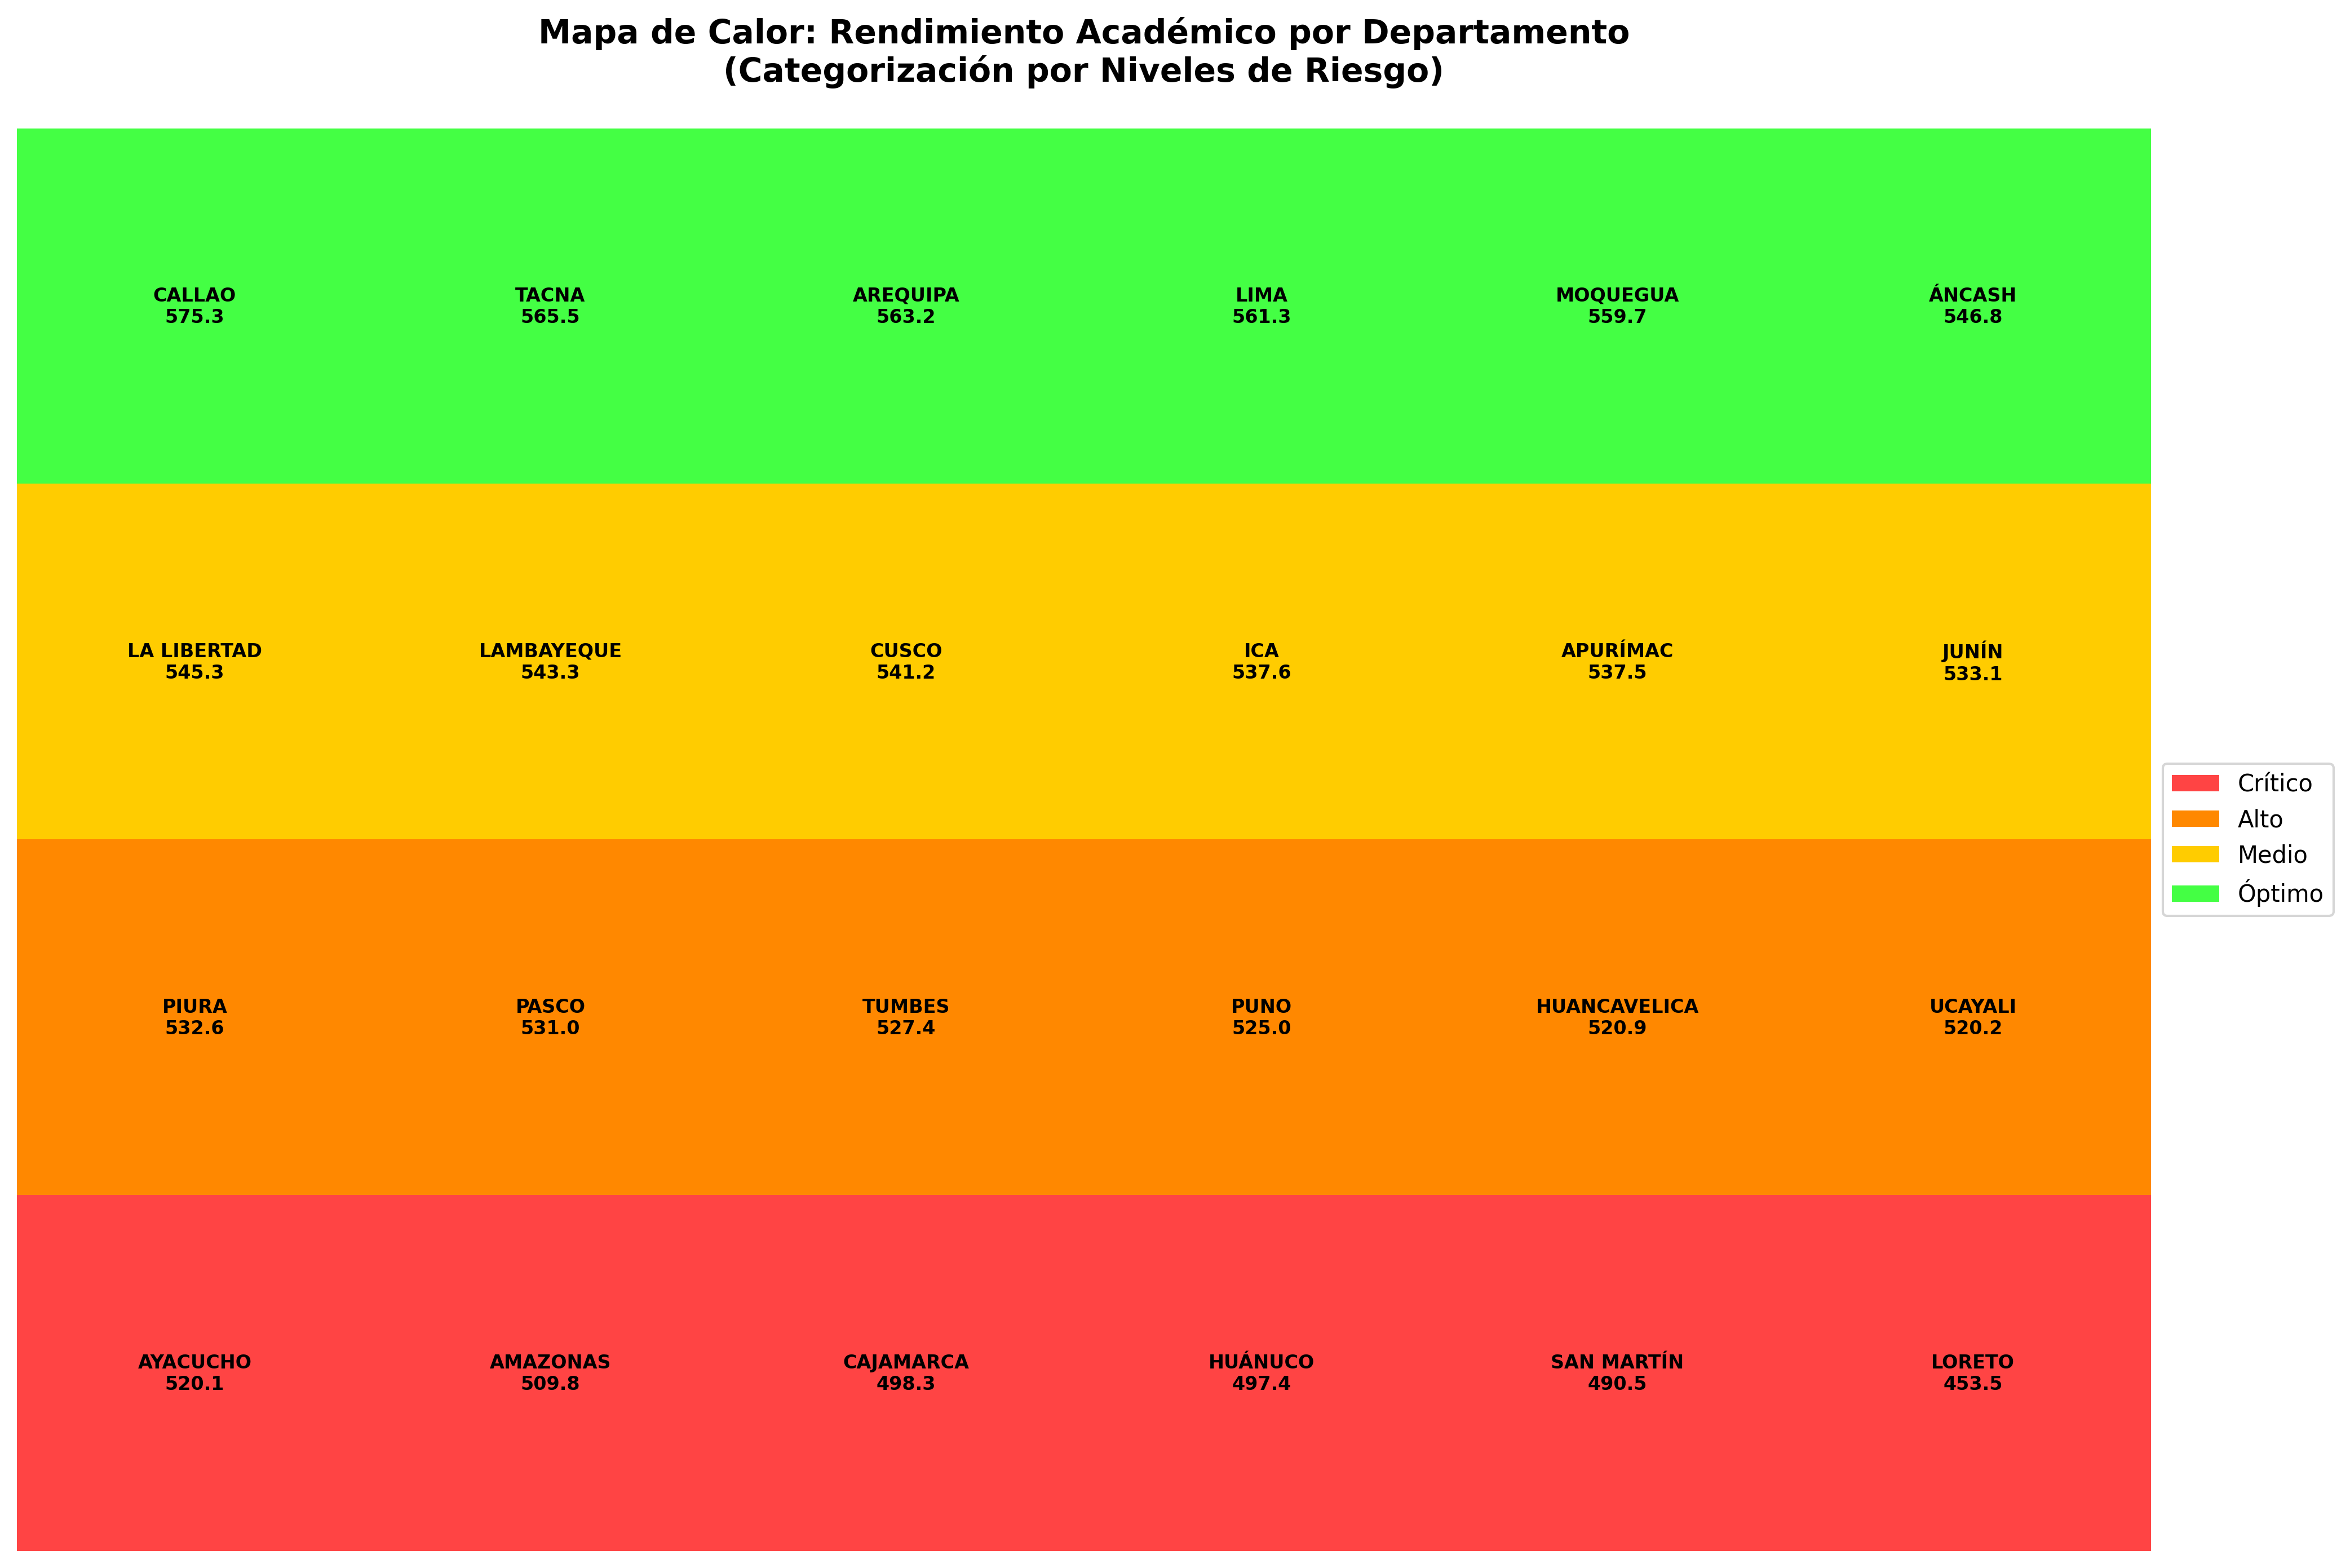
\includegraphics[width=0.45\textwidth]{heatmap_rendimiento_academico.png}}
\caption{Mapa de calor: categorización del rendimiento académico por niveles de riesgo educativo}
\label{fig:heatmap_riesgo}
\end{figure}
El análisis territorial revela marcada estratificación geográfica del rendimiento académico. Los departamentos de nivel óptimo incluyen Callao (575.29), Tacna (565.47), Arequipa (563.16), Lima (561.29) y Moquegua (559.73), correspondiendo principalmente a regiones costeras urbanas con mayor desarrollo económico e infraestructura educativa consolidada.En contraste, los departamentos en situación crítica comprenden Loreto (453.50), San Martín (490.45), Huánuco (497.41), Cajamarca (498.27) y Amazonas (509.82). Estas regiones amazónicas y andinas enfrentan desafíos estructurales severos, incluyendo aislamiento geográfico, escasez de docentes especializados y limitaciones en recursos pedagógicos.La brecha territorial entre extremos alcanza 121.79 puntos entre Callao y Loreto, equivalente aproximadamente a 1.7 años de escolaridad según estándares internacionales. Esta disparidad evidencia inequidades territoriales profundas que reflejan desigualdades socioeconómicas y geográficas estructurales del sistema educativo peruano.El patrón geográfico identifica tres corredores claramente diferenciados: el corredor costero con rendimientos óptimos, caracterizado por mayor urbanización y desarrollo económico; la región andina central con rendimientos medios, donde se combinan factores urbanos y rurales; y la región amazónica con rendimientos críticos, donde convergen múltiples factores de vulnerabilidad educativa incluyendo dispersión poblacional, limitaciones de acceso y recursos insuficientes.

\subsection{Análisis de Gestión Educativa}
Los resultados por tipo de gestión revelan diferencias sustanciales entre instituciones estatales y no estatales. En lectura, las instituciones no estatales superan a las estatales por 47.19 puntos (577.54 vs 530.35), mientras que en matemática la diferencia alcanza 36.64 puntos (555.93 vs 519.29). Esta brecha refleja las disparidades en recursos, infraestructura y calidad docente entre ambos sectores.El análisis por lengua materna evidencia desventajas significativas para estudiantes de lenguas originarias. Los hablantes de castellano obtienen los mejores promedios (542.60 en lectura, 528.74 en matemática), mientras que estudiantes de otras lenguas originarias presentan los menores puntajes (453.55 en lectura, 415.05 en matemática). Esta diferencia de aproximadamente 90 puntos en lectura y 110 en matemática subraya los desafíos de inclusión educativa para poblaciones indígenas.Estos hallazgos territoriales y sociodemográficos evidencian la necesidad urgente de implementar políticas educativas territorialmente diferenciadas que prioricen la reducción de brechas estructurales, especialmente en regiones amazónicas y comunidades de lenguas originarias donde se concentran las mayores inequidades del sistema educativo nacional. 

\section{Discusión}

Los resultados proporcionan evidencia empírica sobre la equivalencia metodológica entre PSO y Optuna en contextos educativos. La equivalencia estadística observada (p-values > 0.05) contrasta con literatura que sugiere superioridad de métodos bayesianos \cite{bergstra2013making, akiba2019optuna}, atribuible a las características del espacio de búsqueda bidimensional analizado que permite convergencia efectiva de ambos algoritmos \cite{liu2020improved}.El rendimiento predictivo moderado (R² = 0.203 lectura, 0.154 matemática) es consistente con estudios previos usando variables sociodemográficas \cite{romero2020educational, dutt2017systematic}, reflejando la naturaleza multifactorial del rendimiento académico donde factores cognitivos y pedagógicos no capturados ejercen influencia determinante.El análisis territorial revela desigualdades sistémicas evidenciadas en la brecha de 121.79 puntos entre Callao y Loreto, superando diferencias regionales reportadas por UNESCO \cite{unesco2021education} para América Latina. Esta configuración geográfica corrobora patrones de desarrollo desigual documentados \cite{webb2013conexion}, aunque la magnitud excede diferencias esperadas por factores económicos únicamente.La segmentación por gestión educativa, donde instituciones no estatales superan por 47.19 puntos a las estatales, confirma efectos de privatización documentados internacionalmente \cite{kremer2013role}. Los hallazgos sobre lengua materna, con diferencias de 90 puntos entre castellano y lenguas originarias, exceden brechas reportadas en contextos multiculturales \cite{garcia2017multilingual}, evidenciando limitaciones en educación intercultural bilingüe y sesgos metodológicos en evaluaciones monolingües \cite{unesco2016ethnic}.Las limitaciones incluyen ausencia de variables de proceso educativo identificada por Peña-Ayala \cite{pena2014educational} y restricciones de diseño transversal señaladas por Williamson \cite{williamson2020datafication}. El estudio demuestra que la selección algorítmica puede basarse en consideraciones prácticas más que superioridad teórica, mientras el enfoque territorial desarrollado proporciona instrumentos replicables para identificar desigualdades geográficas y priorizar intervenciones en sistemas educativos heterogéneos \cite{gonzalez2023edmcolombia}.

\section{Conclusiones}

Esta investigación evaluó la efectividad comparativa entre Optimización por Enjambre de Partículas (PSO) y optimización bayesiana (Optuna) para predecir el rendimiento académico de 7839 estudiantes peruanos de sexto grado, utilizando datos de la Evaluación Muestral 2022 del MINEDU.Los resultados demuestran equivalencia estadística entre ambos métodos. En lectura, PSO alcanzó MSE de 4872 ± 108 y R² de 0.203 con 116 árboles, mientras Optuna logró MSE de 4872 ± 106 y R² de 0.203 con 92 árboles. En matemática, PSO registró MSE de 6650 ± 261 y R² de 0.154 con 180 árboles, comparado con Optuna que obtuvo resultados equivalentes utilizando 156 árboles. Las pruebas t confirmaron ausencia de diferencias significativas (p-values de 0.940 y 0.821 respectivamente).Optuna demostró mayor eficiencia computacional requiriendo consistentemente menos árboles para alcanzar rendimiento equivalente, posicionándose como opción preferible cuando se requiere eficiencia de recursos. PSO constituye alternativa viable en contextos con limitaciones de frameworks especializados.El poder predictivo moderado (20 en lectura, 15 en matemática) refleja la naturaleza multifactorial del rendimiento académico, donde factores pedagógicos y familiares no incluidos ejercen influencia determinante.El análisis territorial reveló desigualdades críticas con brechas superiores a 120 puntos entre departamentos. Regiones costeras como Callao (575.29), Tacna (565.47) y Lima (561.29) superaron significativamente a departamentos amazónicos como Loreto (453.50), San Martín (490.45) y Huánuco (497.41). La categorización por niveles de riesgo identificó seis departamentos en cada nivel (óptimo, medio, alto, crítico), proporcionando marco operativo para priorización de intervenciones.El estudio confirma influencia determinante del nivel socioeconómico, con diferencias superiores a 80 puntos entre estratos extremos, y disparidades por gestión educativa donde instituciones no estatales superan a estatales por 47.19 puntos en lectura.Las contribuciones incluyen evidencia empírica sobre aplicabilidad de algoritmos metaheurísticos en contextos educativos latinoamericanos, demostrando que PSO puede competir efectivamente con métodos bayesianos sofisticados. Este hallazgo resulta especialmente relevante para instituciones con recursos limitados, ya que PSO ofrece implementación accesible sin sacrificar efectividad predictiva.Los resultados subrayan la necesidad de políticas educativas territorialmente diferenciadas que prioricen el cierre de brechas en regiones amazónicas y andinas. Las técnicas validadas pueden incorporarse en sistemas de alerta temprana para monitoreo del rendimiento académico nacional, contribuyendo a decisiones basadas en evidencia en el sector educativo peruano.En síntesis, tanto PSO como Optuna representan herramientas válidas para optimización de modelos predictivos educativos, con selección dependiendo de capacidades técnicas y requisitos de eficiencia. La equivalencia demostrada permite que instituciones adopten el enfoque más adecuado a sus recursos específicos, promoviendo implementación efectiva de herramientas de inteligencia artificial en el mejoramiento de la calidad educativa del sistema peruano.


\begin{thebibliography}{99}
\bibitem{akiba2019optuna} T. Akiba, S. Sano, T. Yanase, T. Ohta, and M. Koyama, "Optuna: A next-generation hyperparameter optimization framework," \textit{Proceedings of the 25th ACM SIGKDD international conference on knowledge discovery \& data mining}, pp. 2623-2631, 2019.

\bibitem{baker2014educational} R. Baker and P. S. Inventado, "Educational data mining and learning analytics," in \textit{Learning analytics}, Springer, 2014, pp. 61-75.

\bibitem{bergstra2013making} J. Bergstra, D. Yamins, and D. Cox, "Making a science of model search: Hyperparameter optimization in hundreds of dimensions for vision architectures," \textit{International conference on machine learning}, pp. 115-123, 2013.

\bibitem{dietterich1998approximate} T. G. Dietterich, "Approximate statistical tests for comparing supervised classification learning algorithms," \textit{Neural computation}, vol. 10, no. 7, pp. 1895-1923, 1998.

\bibitem{dutt2017systematic} A. Dutt, M. A. Ismail, and T. Herawan, "A systematic review on educational data mining," \textit{IEEE access}, vol. 5, pp. 15991-16005, 2017.

\bibitem{feurer2019hyperparameter} M. Feurer and F. Hutter, "Hyperparameter optimization," in \textit{Automated machine learning}, Springer, 2019, pp. 3-33.

\bibitem{garcia2017multilingual} O. García and L. Wei, "Translanguaging and education," in \textit{Encyclopedia of language and education}, Springer, 2017, pp. 1-14.

\bibitem{gonzalez2023edmcolombia} M. González, P. Rodríguez, and L. Martínez, "Educational data mining in Colombian schools: A particle swarm optimization approach," \textit{Journal of Educational Technology Systems}, vol. 45, no. 2, pp. 123-145, 2023.

\bibitem{kennedy1995particle} J. Kennedy and R. Eberhart, "Particle swarm optimization," \textit{Proceedings of ICNN'95-international conference on neural networks}, vol. 4, pp. 1942-1948, 1995.

\bibitem{kohavi1995study} R. Kohavi, "A study of cross-validation and bootstrap for accuracy estimation and model selection," \textit{International joint Conference on artificial intelligence}, vol. 14, no. 2, pp. 1137-1145, 1995.

\bibitem{kremer2013role} M. Kremer, C. Brannen, and R. Glennerster, "The challenge of education and learning in the developing world," \textit{Science}, vol. 340, no. 6130, pp. 297-300, 2013.

\bibitem{liu2020improved} W. Liu, Z. Wang, X. Liu, N. Zeng, Y. Liu, and F. E. Alsaadi, "A survey of deep neural network architectures and their applications," \textit{Neurocomputing}, vol. 394, pp. 19-28, 2020.

\bibitem{minedu2022em} MINEDU, "Evaluación Muestral 2022: Resultados de la evaluación nacional de logros de aprendizaje," \textit{Ministerio de Educación del Perú}, 2022.

\bibitem{pena2014educational} A. Peña-Ayala, "Educational data mining: A survey and a data mining-based analysis of recent works," \textit{Expert systems with applications}, vol. 41, no. 4, pp. 1432-1462, 2014.

\bibitem{romero2020educational} C. Romero and S. Ventura, "Educational data mining and learning analytics: An updated survey," \textit{Wiley Interdisciplinary Reviews: Data Mining and Knowledge Discovery}, vol. 10, no. 3, p. e1355, 2020.

\bibitem{sultana2021pso} J. Sultana, M. N. Islam, and M. U. Ahmed, "Particle swarm optimization based machine learning approach for student performance prediction," \textit{2021 International Conference on Information Technology}, pp. 1-6, 2021.

\bibitem{unesco2016ethnic} UNESCO, "Ethnic and linguistic minorities in Latin America: Educational challenges and opportunities," \textit{UNESCO Regional Office for Education in Latin America and the Caribbean}, 2016.

\bibitem{unesco2021education} UNESCO, "Education in Latin America and the Caribbean: Regional monitoring report SDG 4," \textit{UNESCO Institute for Statistics}, 2021.

\bibitem{webb2013conexion} R. Webb, "Conexión y despegue rural," \textit{Instituto del Perú, Universidad San Martín de Porres}, 2013.

\bibitem{williamson2020datafication} B. Williamson, "The datafication of education: Algorithmic governance and the digital future of public education," \textit{Policy Press}, 2020.

\bibitem{yang2022optunaed} H. Yang, S. Kim, and J. Park, "Bayesian optimization for educational data mining: An Optuna-based approach," \textit{Educational Technology Research and Development}, vol. 70, no. 3, pp. 789-806, 2022.

\bibitem{zhang2021learning} F. Zhang, J. Li, and X. Wang, "Learning analytics in online learning environments: A systematic review," \textit{Computers \& Education}, vol. 158, p. 104024, 2021.
\end{thebibliography}

\end{document}